\section{Appendix}
\subsection{Additional Figures}
\begin{figure}[h]
\begin{subfigure}[t]{0.5\linewidth}
\centering
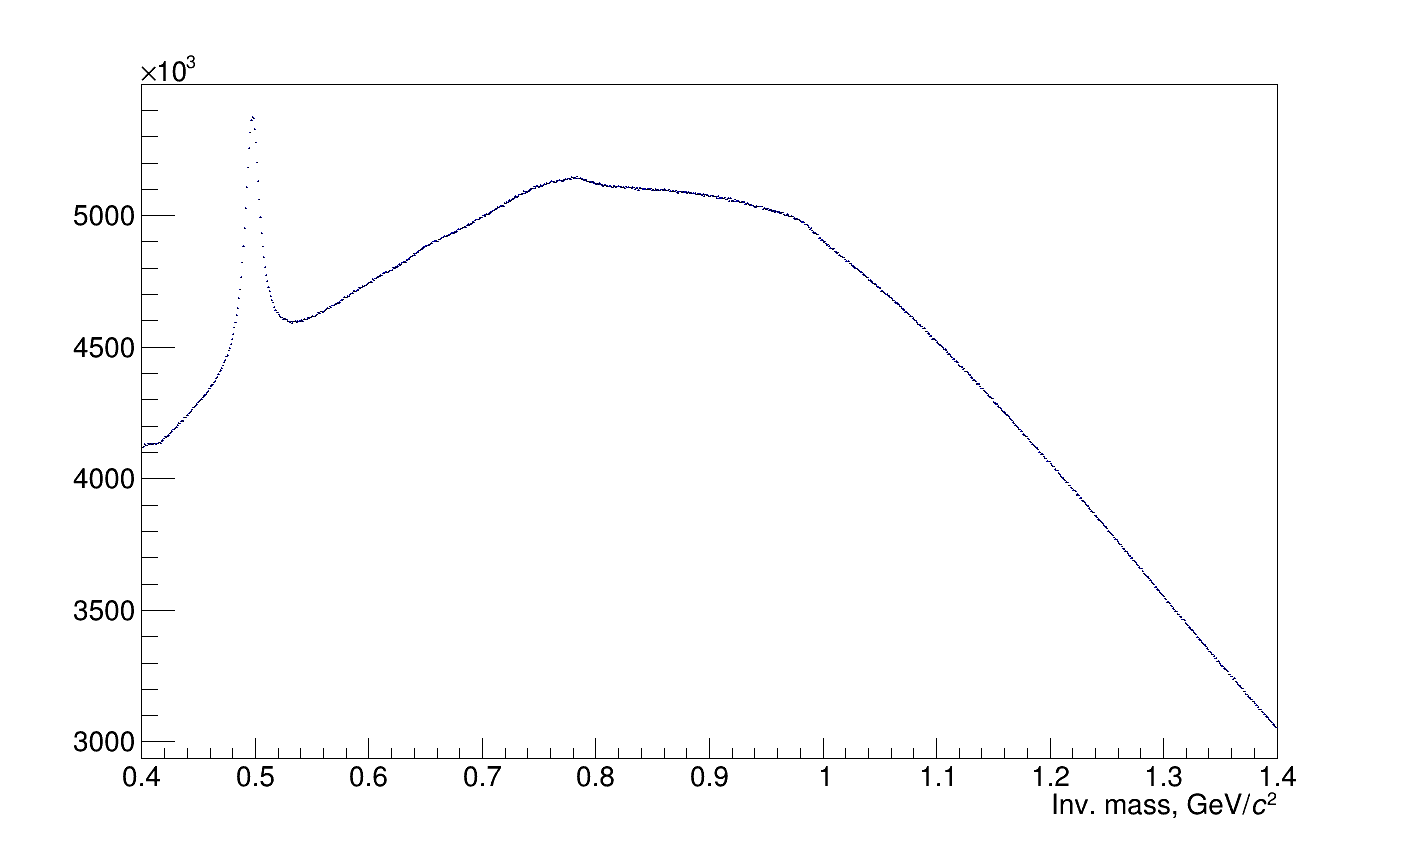
\includegraphics[width=0.98\linewidth]{Figures/ChargedPioSpectra/ChPioMassSpectrum0_25.png}
\caption{Charged Pions Mass Spectrum for $0 \ \mathrm{GeV} \ \leq p_T \leq 2.5 \ \mathrm{GeV}$}
\label{fig:MPtChPio0_25}
\end{subfigure} \hspace{0.1cm}
\begin{subfigure}[t]{.5\linewidth}
\centering
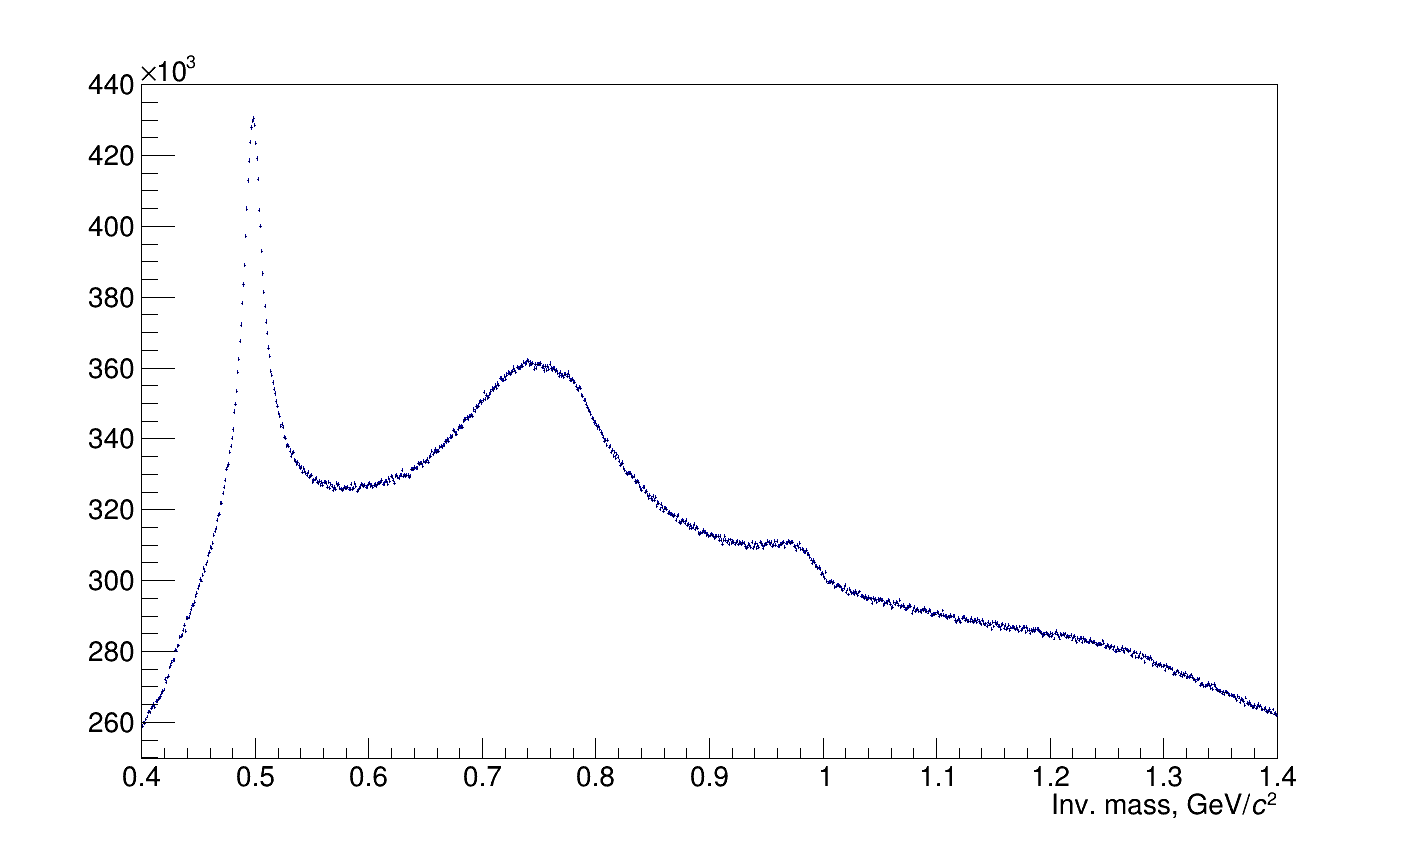
\includegraphics[width=0.98\linewidth]{Figures/ChargedPioSpectra/ChPioMassSpectrum25_50.png}
\caption{Charged Pions Mass Spectrum for $2.5 \ \mathrm{GeV} \ \leq p_T \leq 5.0 \ \mathrm{GeV}$}
\label{fig:MPtChPio25_50}
\end{subfigure}
\begin{subfigure}[t]{0.5\linewidth}
\centering
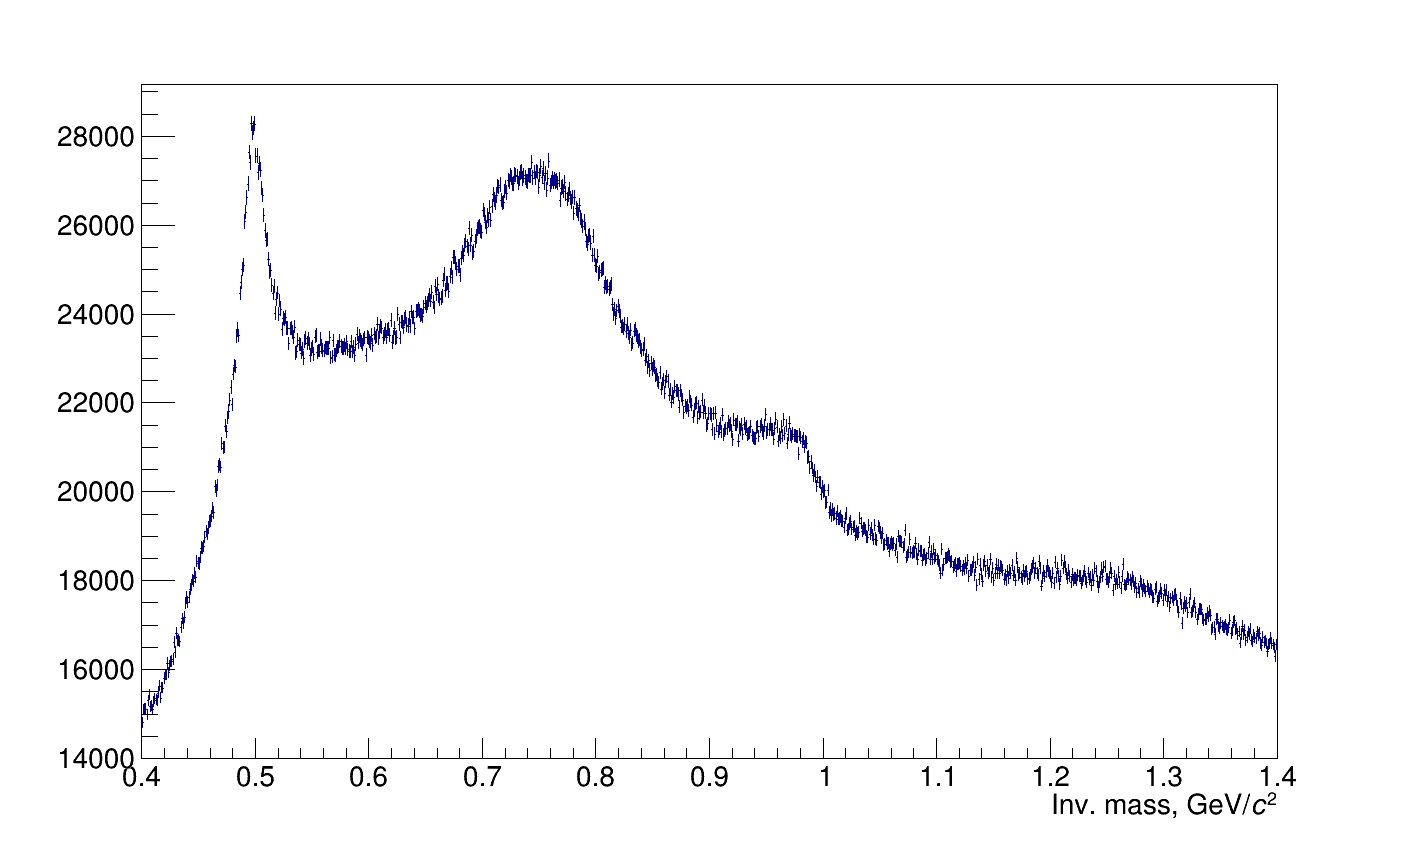
\includegraphics[width=0.98\linewidth]{Figures/ChargedPioSpectra/ChPioMassSpectrum50_75.png}
\caption{Charged Pions Mass Spectrum for $5.0 \ \mathrm{GeV} \ \leq p_T \leq 7.5 \ \mathrm{GeV}$}
\label{fig:MPtChPio50_75}
\end{subfigure} \hspace{0.1cm}
\begin{subfigure}[t]{.5\linewidth}
\centering
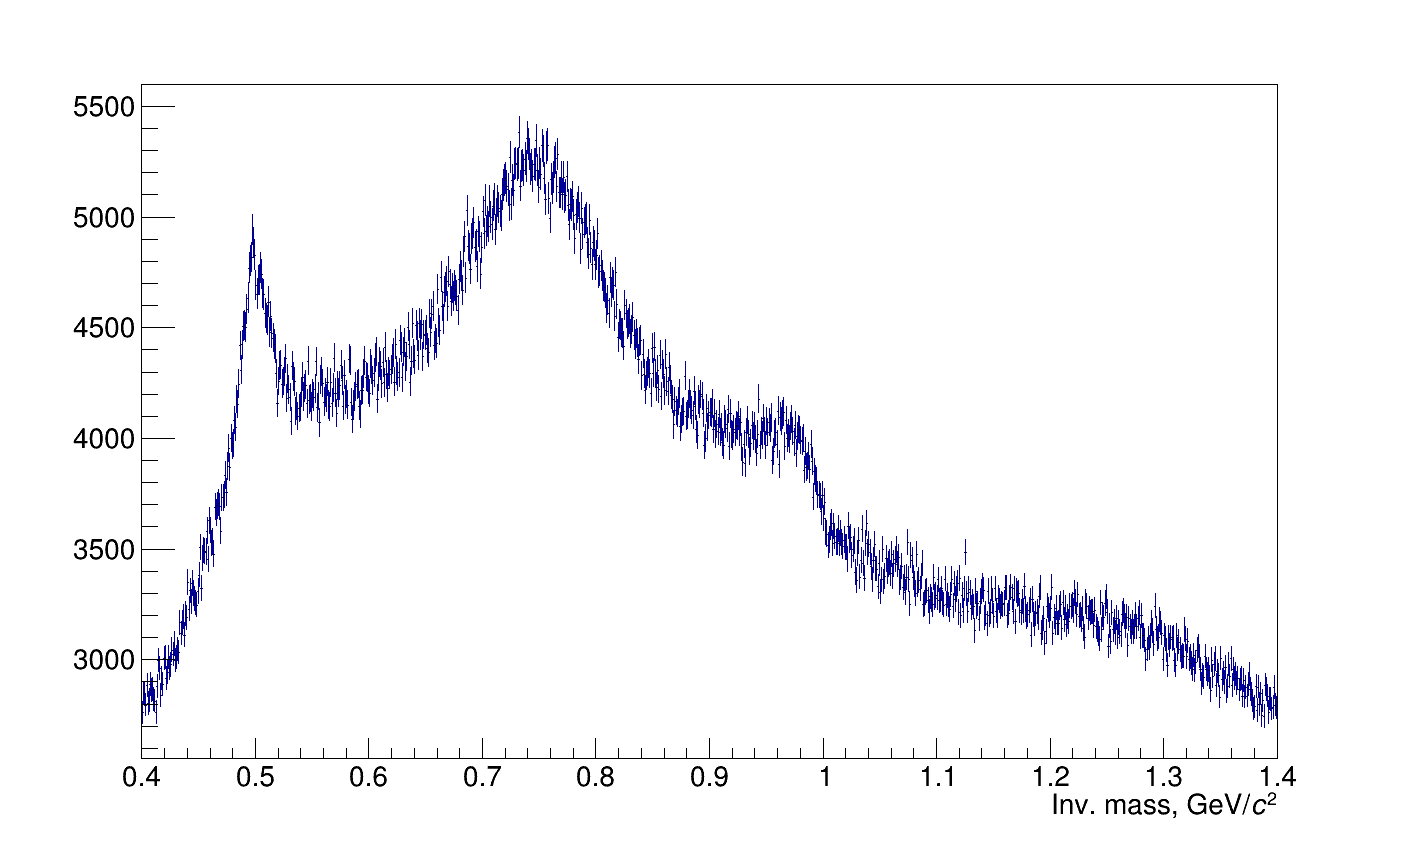
\includegraphics[width=0.98\linewidth]{Figures/ChargedPioSpectra/ChPioMassSpectrum75_100.png}
\caption{Charged Pions Mass Spectrum for $7.5 \ \mathrm{GeV} \ \leq p_T \leq 10.0 \ \mathrm{GeV}$}
\label{fig:MPtChPio75_100}
\end{subfigure}
\begin{subfigure}[t]{0.5\linewidth}
\centering
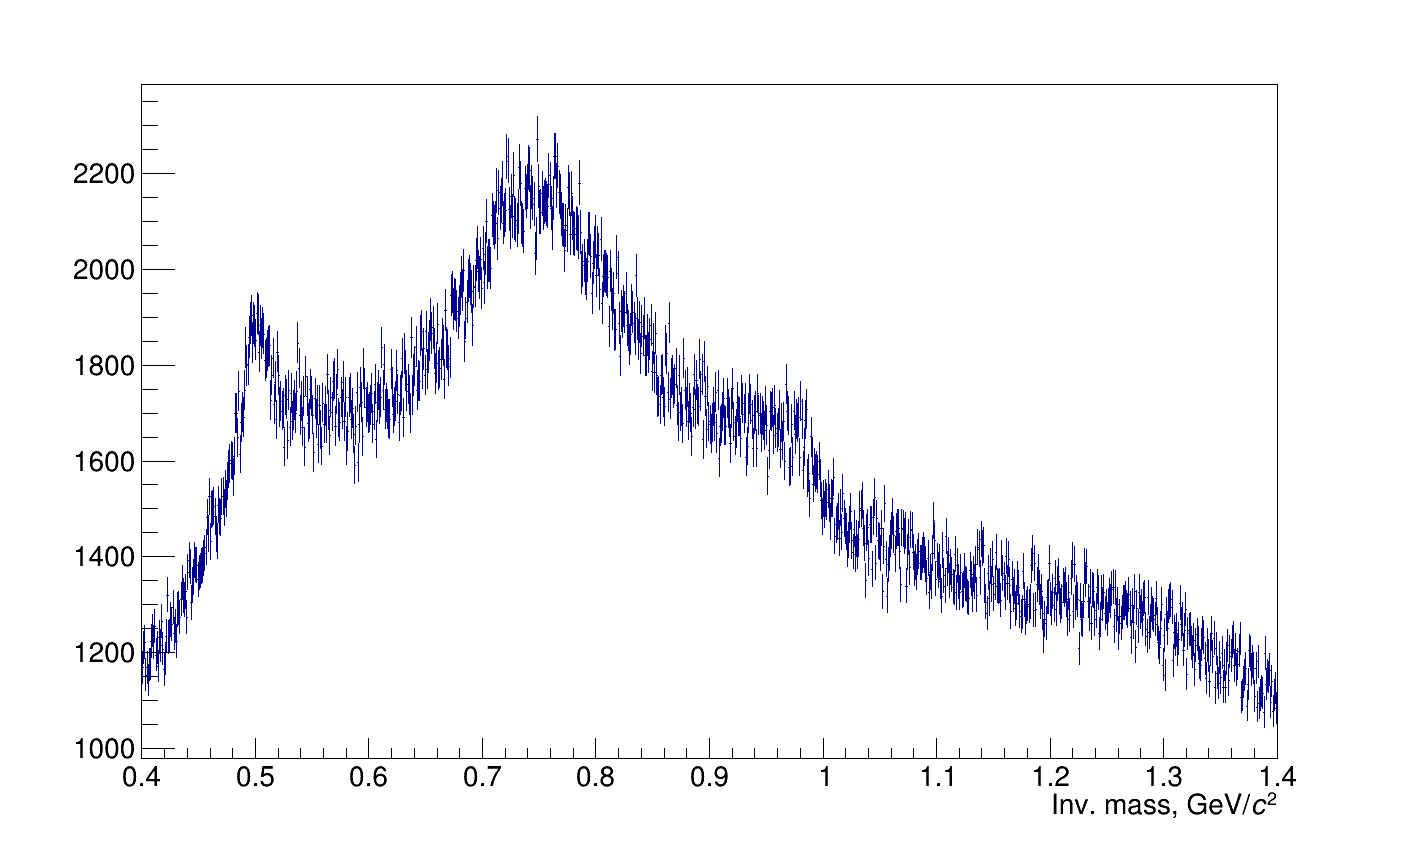
\includegraphics[width=0.98\linewidth]{Figures/ChargedPioSpectra/ChPioMassSpectrum100_150.png}
\caption{Charged Pions Mass Spectrum for $10.0 \ \mathrm{GeV} \ \leq p_T \leq 15.0 \ \mathrm{GeV}$}
\label{fig:MPtChPio100_150}
\end{subfigure} \hspace{0.1cm}
\begin{subfigure}[t]{.5\linewidth}
\centering
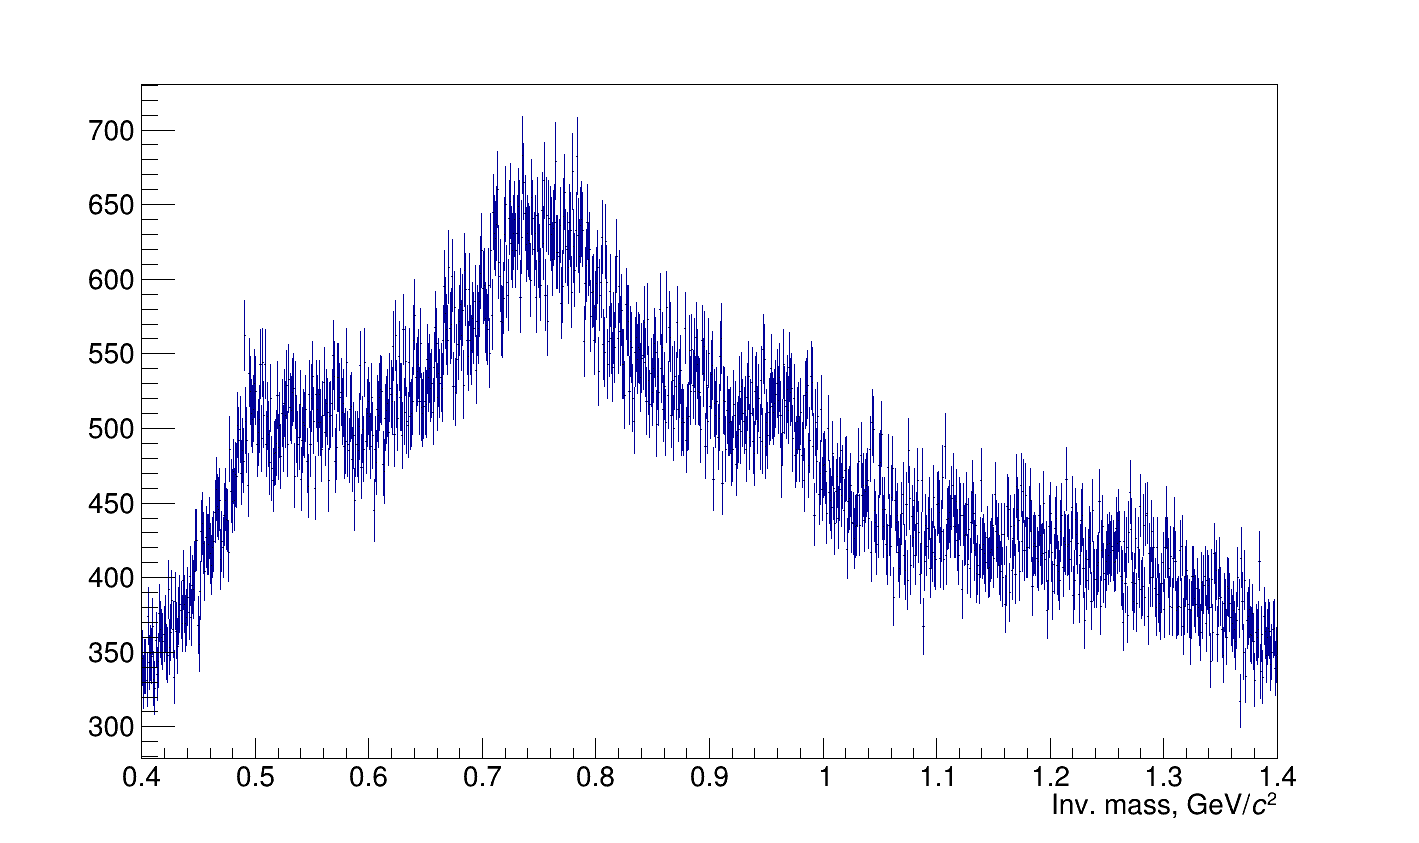
\includegraphics[width=0.98\linewidth]{Figures/ChargedPioSpectra/ChPioMassSpectrum150_1000.png}
\caption{Charged Pions Mass Spectrum for $15.0 \ \mathrm{GeV} \ \leq p_T \leq 100.0 \ \mathrm{GeV}$}
\label{fig:MPtChPio150_1000}
\end{subfigure}
\caption{Mass Spectra of Charged Final State Pions From $\pi^{+} \pi^0\pi^{+}\pi^{-}$ Decay Mode in different $p_T$ windows}
\label{fig:MPtChPio}
\end{figure}